\chapter{Accepttest of SNR}\label{app:journal_Frequency_Response_Noise}
The purpose of this test is verify requirement 9 of the hardware platform, stating that the DSP must comply with IEC 60268-15 and 581-6 standard \citep{IEC60268}. This demands the DSP to have an SNR of > 58 dB. 

\section{Setup}
The setup of this test are depicted in \autoref{fig:AcceptNoise}, where the equipment is catalogued in \autoref{tab:UsedEquipmentAcceptNoise}, and described as follows:

\begin{itemize}
\item Frequency reponse will be measured by a Harmonie 01dB analyzer.
\item No signal we be applied in order to determine the amplitude of the noise which is directly translated as the SNR
\item The software of the system test is found at \path{CD://Software/SystemFinal}
\item The measurements are averaged over a period of 20 seconds.
\end{itemize}


\subsection*{Test Setup}
\begin{figure}[H]
\centering
\includegraphics[width=0.9\textwidth]{FreqReponseSetup1.png}
\caption{Test setup.}
\label{fig:AcceptNoise}
\end{figure}

\subsection*{Equipment used and AAU-no.}

\begin{table}[H]
\centering
\ra{1.3}
\begin{tabular}{S[table-format=1]ccc} \toprule
    {Item} & {Description} & {AAU-no} \\ \bottomrule 
    1      &  Harmonie 01dB  & 60923  \\ 
    2      &  Fujitsu Siemens LifeBook with Harmonie software  & 56524  \\ 
    3      &  TMS320C5515 eZdsp USB stick  & NaN  \\  \bottomrule 
\end{tabular}
\caption{Table over equipment used in the test}
\label{tab:UsedEquipmentAcceptNoise}
\end{table}
\vspace{-5mm}


\section{Procedure}
The procedure for this experiment is described as follows:
\vspace{-5mm}
\begin{enumerate}
\item Setup the Harmonie and the Harmonie PC
\item Start recording on the PC with an average of 20 seconds on each recording
\item When finished save the results of the test.
\item Run trials for both the developed system and a Looped signal
\end{enumerate}

\section{Data Extraction}
The raw data the system can be found at the CD, \\
 \path{CD://Maalinger/Maalinger200516 - Acceptance test for SNR}\\
There are 30 bands from 20 Hz to 20 kHz, see \autoref{tb:freqBandsAppendixNoise}, where a magnitude is given in dB for each band. One measurement have been taken for both the bypass and the full system. The value was sampled over a period of 20 seconds. The mean for each measurement has been calculated. The two bands 25 Hz and 20000 Hz has been removed from the plots because of large deviation and therefore not deemed useful. 

\begin{table}[H]
\centering
\begin{tabular}{|c|c|c|c|c|c|c|c|c|c|}
\hline
\multicolumn{10}{|c|}{Bands [Hz]}                                       \\ \hline
25   & 31.5 & 40   & 50   & 63   & 80   & 100   & 125   & 160   & 200   \\ \hline
250  & 315  & 400  & 500  & 630  & 800  & 1000  & 1250  & 1600  & 2000  \\ \hline
2500 & 3150 & 4000 & 5000 & 6300 & 8000 & 10000 & 12500 & 16000 & 20000 \\ \hline
\end{tabular}
\caption{Frequency bands.}
\label{tb:freqBandsAppendixNoise}
\end{table}

\section{Analysis}
The discrete values from the test are plotted according to their frequency and showed in figure \ref{fig:FFreqNoiseComp}.
\begin{figure}[H]
	\centering
	\tikzsetnextfilename{FreqNoiseComp}
	% This file was created by matlab2tikz.
%
%The latest updates can be retrieved from
%  http://www.mathworks.com/matlabcentral/fileexchange/22022-matlab2tikz-matlab2tikz
%where you can also make suggestions and rate matlab2tikz.
%
\definecolor{mycolor1}{rgb}{0.00000,0.44700,0.74100}%
\definecolor{mycolor2}{rgb}{0.85000,0.32500,0.09800}%
%
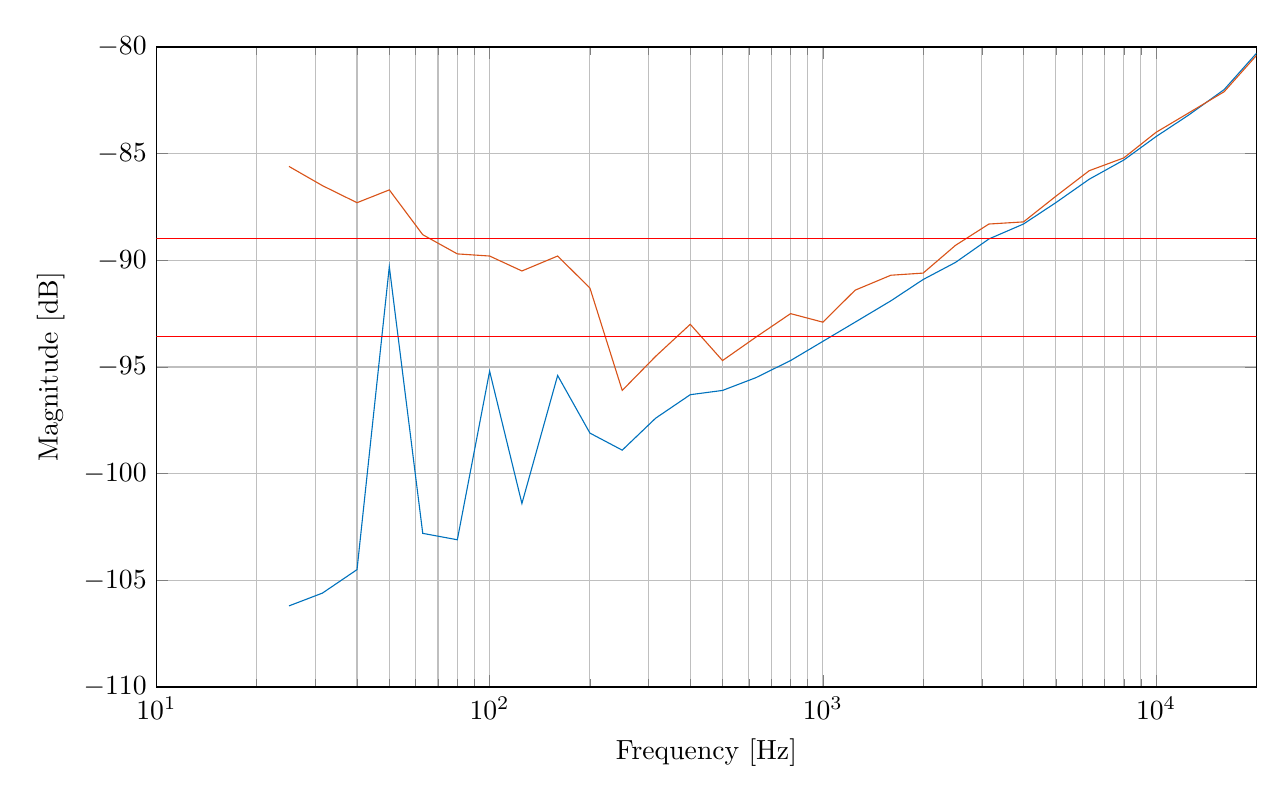
\begin{tikzpicture}

\begin{axis}[%
width=5.5in,
height=3.2in,
at={(0.758in,0.481in)},
scale only axis,
xmode=log,
xmin=10,
xmax=20000,
xminorticks=true,
xlabel={Frequency [Hz]},
xmajorgrids,
xminorgrids,
ymin=-110,
ymax=-80,
ylabel={Magnitude [dB]},
ymajorgrids,
axis background/.style={fill=white}
]
\addplot [color=mycolor1,solid,forget plot]
  table[row sep=crcr]{%
25	-106.2\\
31.5	-105.6\\
40	-104.5\\
50	-90.3\\
63	-102.8\\
80	-103.1\\
100	-95.2\\
125	-101.4\\
160	-95.4\\
200	-98.1\\
250	-98.9\\
315	-97.4\\
400	-96.3\\
500	-96.1\\
630	-95.5\\
800	-94.7\\
1000	-93.8\\
1250	-92.9\\
1600	-91.9\\
2000	-90.9\\
2500	-90.1\\
3150	-89\\
4000	-88.3\\
5000	-87.3\\
6300	-86.2\\
8000	-85.3\\
10000	-84.2\\
12500	-83.2\\
16000	-82\\
20000	-80.3\\
};
\addplot [color=mycolor2,solid,forget plot]
  table[row sep=crcr]{%
25	-85.6\\
31.5	-86.5\\
40	-87.3\\
50	-86.7\\
63	-88.8\\
80	-89.7\\
100	-89.8\\
125	-90.5\\
160	-89.8\\
200	-91.3\\
250	-96.1\\
315	-94.5\\
400	-93\\
500	-94.7\\
630	-93.6\\
800	-92.5\\
1000	-92.9\\
1250	-91.4\\
1600	-90.7\\
2000	-90.6\\
2500	-89.3\\
3150	-88.3\\
4000	-88.2\\
5000	-87\\
6300	-85.8\\
8000	-85.2\\
10000	-84\\
12500	-83.1\\
16000	-82.1\\
20000	-80.4\\
};
\addplot [color=red,solid,forget plot]
  table[row sep=crcr]{%
10	-93.5633333333333\\
100000	-93.5633333333333\\
};
\addplot [color=red,solid,forget plot]
  table[row sep=crcr]{%
10	-88.98\\
100000	-88.98\\
};
\end{axis}
\end{tikzpicture}%
	\caption{Frequency reposnse of bypassed noisefloow (blue) and full system noise floor (orange). Mean bypass=-93.5633, Mean system=-88.98.}
	\label{fig:FFreqNoiseComp}
\end{figure}

From the measurements a mean for both the bypassed system and the full system is derived to be,
\begin{itemize}
	\item Mean bypass=-93.5633 dB
	\item Mean system=-88.98 dB
\end{itemize}

\section{Error sources}

Due to large deviations in the 25 Hz and 20 kHz region, the measurements for these bands have been discarded. However since the IEC 581-6 demands only and effective frequency spectrum of 40 Hz to 16 kHz, the measurements are still deemed valid.

\section{Conclusion}
From the test of the bypass and full system it can be concluded that the SNR is sufficiently high to accept the demands of the IEC 581-6 and 268-3 Standards. 